\section{Calibrazione}
La calibrazione del ricevitore a 1.4 a GHz viene effettuata utilizzando due sorgenti di riferimento, che sono due carichi coassiali adattati, cioè due resistenze a 50 $\Omega$. Questi lavorano a due temperature diverse: uno a temperatura ambiente (\textit{warm load}) e l'altro alla temperatura di ebollizione dell'azoto liquido, ovvero 77,36 K (\textit{cold load}). \\\\Il carico a temperatura criogenica è connesso al ricevitore tramite un cavo coassiale il quale è immerso parzialmente nell'azoto liquido. Perciò, dato che la temperatura del cavo non è uniforme, ne vanno studiate le caratteristiche di attenuazione in laboratorio, su un cavo analogo, a temperatura ambiente ed a temperatura criogenica. Per farlo si utilizza un analizzatore vettoriale di reti (VNA).

\subsection{Attenuazione cavo coassiale}
Il cavo Cold Load che viene utilizzato nella calibrazione del ricevitore è solo parzialmente immerso nell'azoto liquido, la sua temperatura non è quindi costante. Perciò, il coefficiente di attenuazione del cavo viene misurato con il VNA sia a temperatura ambiente, sia a temperatura criogenica. Per farlo si utilizza un cavo di rame analogo di forma elicoidale, così da facilitarne l'immersione nell'azoto, e di lunghezza 203 cm. 

\begin{figure}[h]
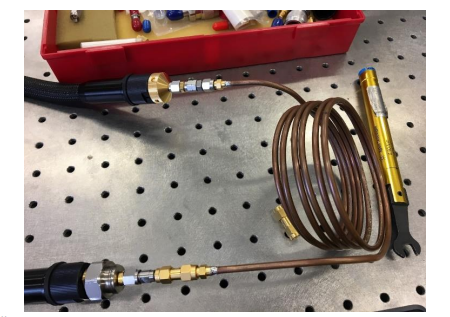
\includegraphics[scale=0.60]{cavo rame.png}
\centering
\caption{Cavo di rame collegato alle porte del VNA}
\label{fig:Cavo di rame}
\end{figure}

Il rame, però, ha una conducibilità termica molto elevata. Per questo motivo, al fine di prottegere il VNA ed evitare che i suoi cavi lavorino ad una temperatura di 77,36 K, si utilizzano dei separatori termici. Essi stessi tuttavia attenuano il segnale. Viene quindi effettuata una misura intermedia dell'attenuazione dei separatori, collegandoli tra loro. In questo modo è poissibile togliere il loro contributo dal calcolo del coefficiente di attenuazione del cavo di rame.
\subsubsection{VNA e parametri di scattering}
Il VNA è una macchina che permette di misurare le proprietà di trasmissione di un cavo coassiale i cui estremi sono connessi ai terminali dello strumento. Il VNA presente il laboratorio è un Agilent PNA-X che è in grado di misurare in modo indipendente il segnale di trasmissione e riflessione dalle due porte presenti.
\begin{figure}[h]
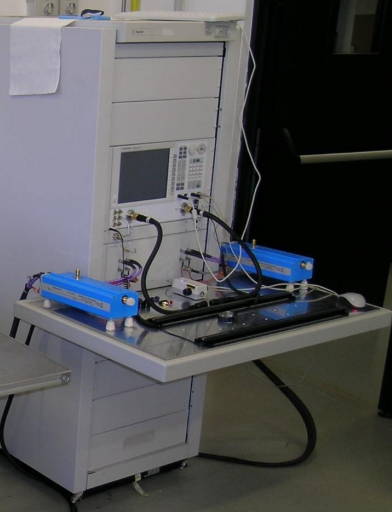
\includegraphics[scale=0.60]{VNA.png}
\centering
\caption{VNA presente in laboratorio. Il modello è un Agilent PNA-X.}
\label{fig:VNA}
\end{figure}

Quindi ciò che la macchina restituisce è la cosiddetta matrice di scattering i cui parametri sono: i coefficienti di riflessione, \textit{$s_{11}$} e \textit{$s_{22}$}, ed i coefficienti di trasmissione, \textit{$s_{12}$} e \textit{$s_{21}$}. Dove vale che:\\\\
\begin{equation}
    s_{11}=10\log_{10} \frac{Potenza\,\,riflessa\,\,nella\,\,porta\,\,1}{Potenza\,\,incidente\,\,dalla\,\,porta\,\,1},
\end{equation}
\begin{equation}
    s_{12}=10\log_{10} \frac{Potenza\,\,trasmessa\,\,dalla\,\,porta\,\,1\,\,alla\,\,porta\,\,2}{Potenza\,\,incidente\,\,dalla\,\,porta\,\,1},
\end{equation}
\begin{equation}
    s_{21}=10\log_{10} \frac{Potenza\,\,trasmessa\,\,dalla\,\,porta\,\,2\,\,alla\,\,porta\,\,1}{Potenza\,\,incidente\,\,dalla\,\,porta\,\,2},
\end{equation}
\begin{equation}
    s_{22}=10\log_{10} \frac{Potenza\,\,riflessa\,\,nella\,\,porta\,\,2}{Potenza\,\,incidente\,\,dalla\,\,porta\,\,2};
\end{equation}
\\NON SO SE METTERE QUESTA PARTE
Impostiamo che la macchina lavori in una banda di frequenza che varia dai 500 MHz ai 3 GHz e che faccia una scansione in frequenza in 201 punti e con una potenza di 0 dB. Per calibrare la macchina è necessario togliere l’effetto dei cavi di misura: per farlo si danno, tramite calibratore elettronico, degli standard di riferimento: lo standard di riflessione totale e lo standard di trasmissione e di sfasamento. In questo modo viene calcolato l’error box della macchina, cioè la matrice di compensazione dell’effetto dei cavi.


\subsubsection{Matrice di scattering con separatori termici}

I separatori termici vengono connessi tra loro tramite degli adattatori, tramite tale processo è possibile ricavare i coefficienti di trasmissione, $ s_{21} $, e riflessione, $ s_{11} $, a temperatura ambiente e temperatura criogenica, rispettivamente $ T_{A}\sim290K $ e $ T_{C} \sim77.36K $. Più dettagliatamente:

\begin{itemize}
\item s11: si instaurano onde stazionarie durante il percorso. Sono presenti dei minimi e dei massimi, quindi a determinare lunghezze d'onda il segnale avrà riflessione massima o minima, ma comunque inferiore all'1 \% del segnale;
\item s21: anche in questo caso sono presenti oscillazioni, con un'attenuazione di 0.4 dB.
\end{itemize}

\begin{figure}[h]
\centering

\begin{subfigure}{0.49\textwidth}
	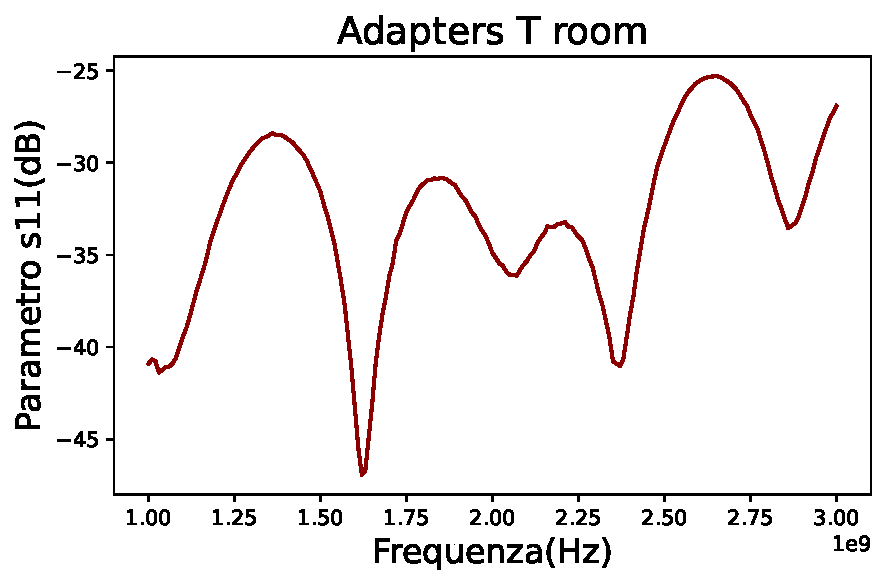
\includegraphics[width=\textwidth]{S11_TA.pdf}
    \caption{$s_{11}$ separatori termici a $T_{A}$}
    \label{fig:sub1}
\end{subfigure}
\hfill
\begin{subfigure}{0.49\textwidth}
    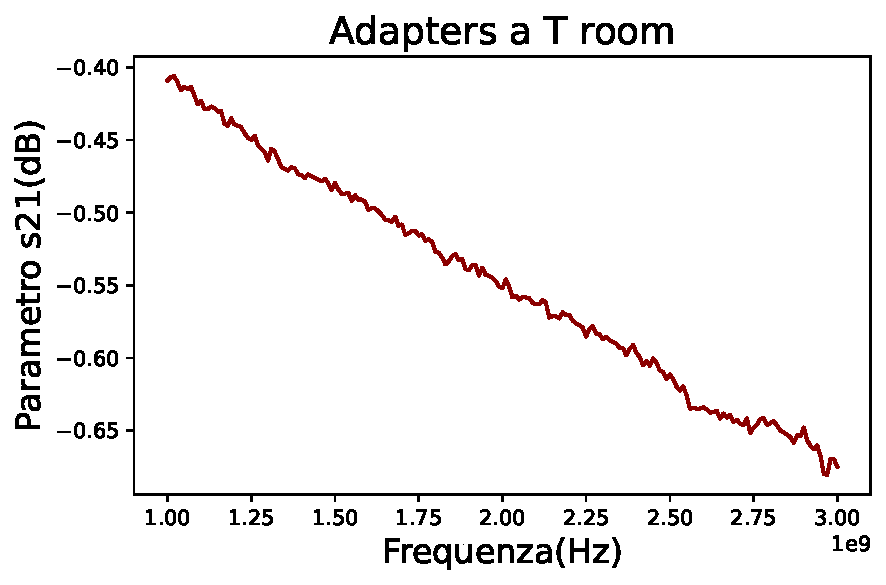
\includegraphics[width=\textwidth]{S21_TA.pdf}
    \caption{$s_{21}$ separatori termici a $T_{C}$}
    \label{fig:sub2}
\end{subfigure}

\end{figure}

\subsubsection{Matrice di scattering con separatori termici e cavo di rame}

\subsubsection{Matrice di scattering del cavo di rame}

\subsubsection{Calcolo del coefficiente di attenuazione}
\label{ssec:Calcolo del coefficiente di attenuazione}

\subsection{Calibrazione del ricevitore a 1.4 GHz}

La conoscenza del profilo del coefficente di attenuazione in funzione della temperatura permette di attuare la calibrazione del ricevitore a 1,4 GHz. Si consideri come warm load e cold load, un cavo rispettivamente di lunghezza 12 m e 120 cm. Il cold load è immerso parzialmente nell'azoto liquido portando ad un'attenuazione del segnale.\\
Per ottenere il segnale effettivo letto dal ricevitore è quindi necessario considerare la variazione della temperatura all'interno del cavo.

\subsubsection{Profilo di temperatura del cavo}
\label{ssec:Profilo di temperatura del cavo}

La stima del profilo di temperatura è resa possibile grazie a 4 sensori criogenici e 2 sensori a temperatura ambiente posizionati sul cavo, come mostrato in figura \ref{fig:cavi}. 

\begin{figure}[h]
\centering

	\begin{subfigure}{0.49\textwidth}
		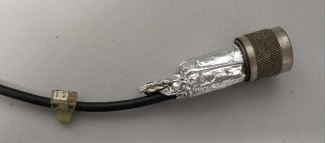
\includegraphics[width=\textwidth]{Posizione_sensori_1.png}
    		\caption{Uno dei sensori connesso al cavo warm load}
   	 	\label{fig:sub1}
	\end{subfigure}
	\hfill
	\begin{subfigure}{0.49\textwidth}
		\centering
    		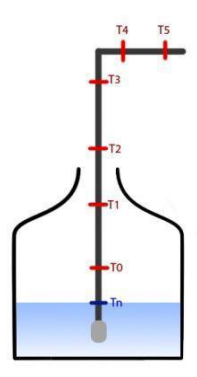
\includegraphics[width=0.5\textwidth]{Posizione_sensori_3.png}
    		\caption{Schema della posizione dei cavo durante l'immersione nell'azoto}
    		\label{fig:sub2}
	\end{subfigure}

	\begin{subfigure}{0.49\textwidth}
		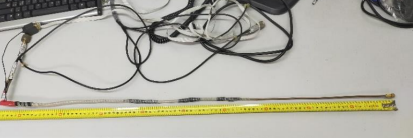
\includegraphics[width=\textwidth]{Posizione_sensori_2.png}
    		\caption{Uno dei sensori connesso al cavo warm load}
    		\label{fig:sub3}
	\end{subfigure}
	\hfill
	\begin{subfigure}{0.49\textwidth}
    		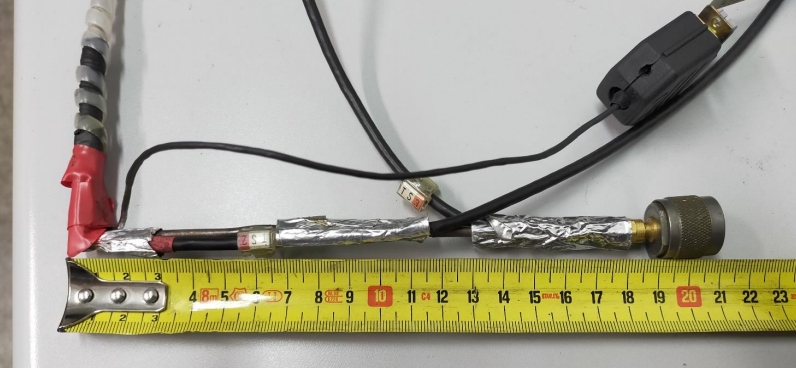
\includegraphics[width=\textwidth]{Posizione_sensori_4.png}
    		\caption{Schema della posizione dei cavo durante l'immersione nell'azoto}
    		\label{fig:sub4}
	\end{subfigure}

\caption{Visualizzazione grafica dei rilevatori sul cavo}
\label{fig:cavi}
\end{figure}


I primi 4 sensori restituiscono il valore in Kelvin, mentre gli ultimi due attuano la loro misurazione in gradi Celcius.\\
Successivamente all' immersione completa del cold load nel criostato che contiene Azoto liquido a pressione ambiente. Dai valori ottenuti dai sensori è quindi possibile determinare l'andamento della temperatura in funzione della posizione. 

\begin{table}
\centering

\begin{tabular}{ |c|c|  }
	\hline
	\multicolumn{2}{|c|}{Valori di temperatura registrati nella posizione del sensore} \\
	\hline
	Posizione (mm)& Temperatura (K) \\
	\hline
	295   & 77,36    \\
	380  & 110,2  \\
	480 &197,3 \\
	610    &264,3 \\
	910&   296,0  \\
	1030& 295,8  \\
	1110& 296.2  \\
	\hline
\end{tabular}

\end{table}

Infine, si fittino i seguenti valori con una funzione sigmoide:
\begin{equation}
T= \dfrac{a}{1+e^{-k(x-x_{0})}},
\end{equation}
Il grafico che si ottiene è il seguente:
\begin{figure}[h]
	\centering
	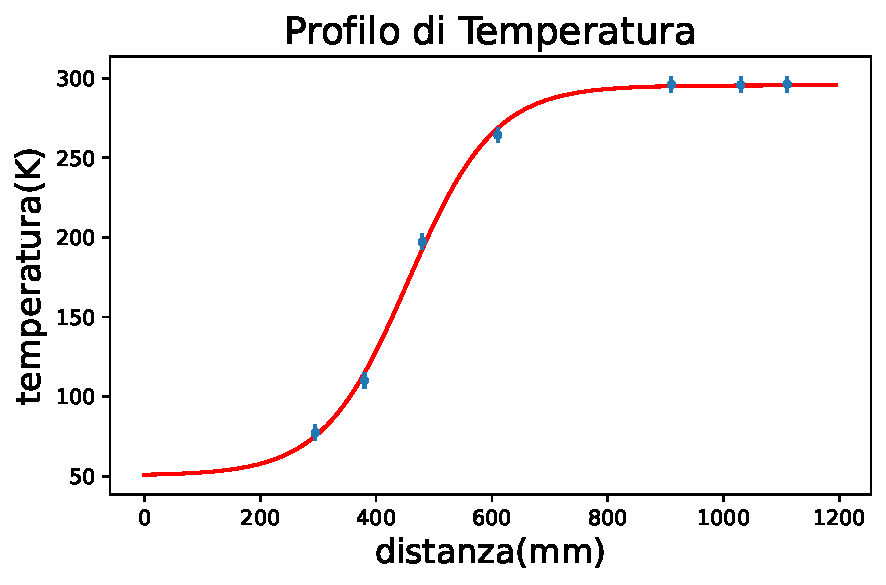
\includegraphics[scale=0.8]{Profilo_temperatura.pdf}
	\caption{Fit del profilo di temperatura}
    	\label{fig:Profilo_temperatura}
\end{figure}
Successivamente, si ricava dal profilo di  temperatura e dall'andamento del coefficiente di attenuazione in funzione della temperatura il valore di temperatura del cavo cold load e warm load.


\subsubsection{Temperatura del cavo cold load}
\label{ssec:Temperatura del cavo cold load}

L'immersione parziale del cavo cold load all'interno del criostato comporta che la temperatura del carico criogenico deve essere corretta. La propagazione della temperatura nel cavo segue il seguente andamento:

\begin{equation}
T_{b}= T_{s}e^{-\tau} + T_{C}(1-e^{-\tau}),
\label{Formula ricorsiva}
\end{equation}

dove $T_{s}$ è pari a 77,36 K, ovvero la temperatura di ebolizione dell'azoto liquido, $T_{c}$ è il valore della temperatura studiata nel paragrafo \ref{ssec:Profilo di temperatura del cavo} e $\tau$ è il coefficiente di attenuazione studiato nel paragrafo \ref{ssec:Calcolo del coefficiente di attenuazione}.
Si applichi tale relazione iterativamente a dei tratti di lunghezza $\Delta$x. Lo step di lunghezza viene scelto in modo tale da poter considerare il tratto di cavo preso in considerazione isotermo. Si scelga quindi un valore di $\Delta$x = 1 mm.
L'iterazione dell'equazione \eqref{Formula ricorsiva} è dovuta al fatto che il sistema risulta essere in equilibrio per tutto il tratto di cavo immerso nell'azoto liquido. \`E quindi possibile considerare valida la relazione $T_{b} = T_{s} = 77,36 K$. Nel tratto di cavo scoperto il sistema non è più all'equilibrio, la temperatura del cavo varia ed è quindi necessario determinare il coefficiente di attenuazione $\tau$ del cavo.\\
Successivamente a tali considerazioni si ricava un valore di $T_{b}$ = 91,95 K.

\begin{figure}[h]
	\centering
	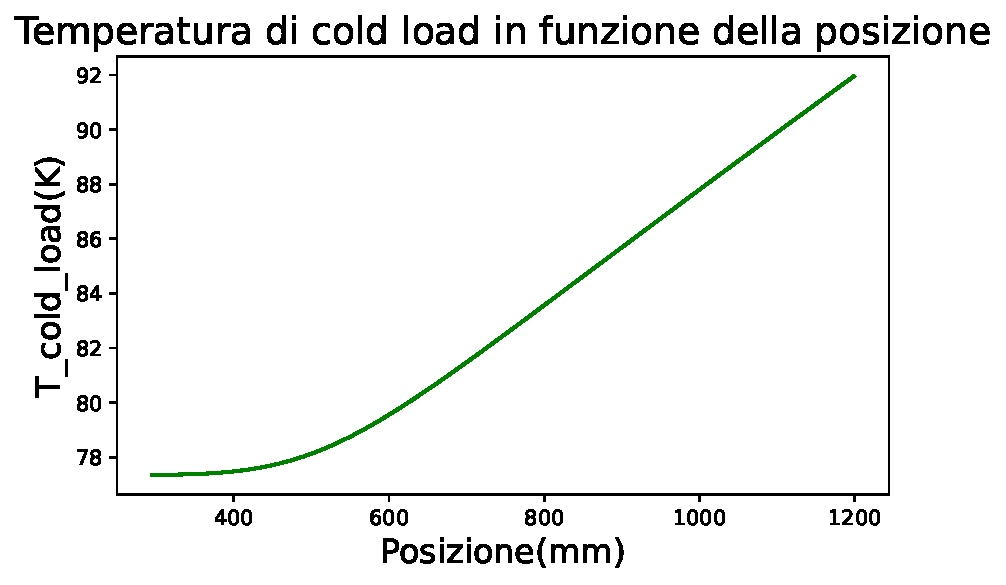
\includegraphics[scale=0.8]{Temperatura_vs_posizione.pdf}
	\caption{Andamento della temperatura di cold load in funzione della posizione}
    	\label{fig:Temperatura_vs_posizione}
\end{figure}

%\cite{Cold load:Cold load}.

\subsubsection{Temperatura del cavo warm load}

Per determinare la temperatura del cavo warm load il procedimento è simile a quello utilizzato nel paragrafo \ref{ssec:Temperatura del cavo cold load} con la differenza che la totalità del cavo è a temperatura ambiente. Quindi la sorgente e il cavo hanno circa la stessa temperatura $T_{s}$ $\sim$ $T_{c}$ $\sim$ 273,15 K.\\
Di conseguenza risulta possibile semplificare l'equazzione \eqref{Formula ricorsiva} nel seguente modo:
(da riguardare la formula perchè quella della relazione dell'amica di Simo è sbagliata.)

\subsubsection{Guadagno del ricevitore}
\subsubsection{Temperatura di rumore}
